Le tecniche di embedding costituiscono un pilastro essenziale nel Trattamento del Linguaggio Naturale (Natural Language Processing, NLP). Queste metodologie convertono le parole e i testi in rappresentazioni numeriche, consentendo alle macchine di trattare il linguaggio umano in formato comprensibile. Dall'introduzione di Word2Vec a soluzioni più avanzate come BERT e GPT, il campo delle tecniche di embedding ha segnato un'evoluzione significativa.

\subsubsection{Word2Vec: Catturare il contesto}
Word2Vec, introdotto da Mikolov et al. nel 2013, ha svolto un ruolo cruciale nell'evoluzione delle rappresentazioni vettoriali. Questa tecnica adotta un approccio basato sulla predizione del contesto: attraverso l'analisi delle parole circostanti, Word2Vec crea embedding che catturano le relazioni semantiche tra le parole. Questi embedding sono capaci di rappresentare sinonimi e relazioni tra parole simili.
\begin{center}
    \begin{figure}[H]
        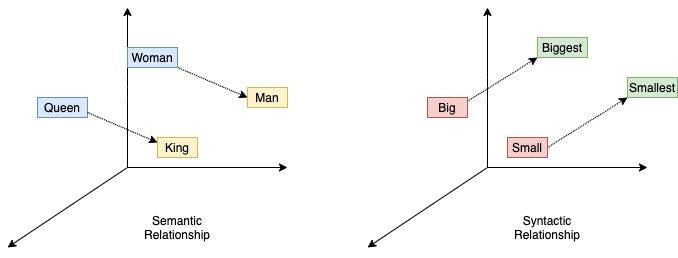
\includegraphics[width=0.6\pdfpagewidth]{images/semanticandsintatic.jpg}
        \caption{La differenza tra un'associazione semantica e una sintattica}
    \end{figure}    
\end{center}

\subsubsection{GloVe: Combattere l'ambiguità}
Il Global Vectors for Word Representation (GloVe \cite{glove}) è un altro approccio popolare all'embedding di parole. Introdotto da Pennington et al. nel 2014, GloVe cerca di superare l'ambiguità linguistica basandosi sulla co-occorrenza delle parole. Questa tecnica considera la frequenza con cui due parole appaiono insieme nel testo, creando embedding che riflettono le relazioni statistiche tra le parole.

\subsubsection{Modelli Transformer: Contesti complessi}
L'introduzione dei modelli Transformer, con BERT e GPT in prima linea, ha segnato un'ulteriore avanzamento nel campo delle rappresentazioni vettoriali. Questi modelli si basano sull'architettura di auto-attenzione, consentendo loro di catturare relazioni contestuali complesse tra le parole. BERT, ad esempio, addestra una rete neurale a prevedere parole mancanti in una frase, generando embedding che riflettono una profonda comprensione del contesto.

\subsubsection{Utilizzo dei modelli pre-addestrati}
Un aspetto cruciale delle tecniche di embedding è l'uso di modelli pre-addestrati. Questi modelli, addestrati su grandi dataset, catturano una vasta gamma di relazioni linguistiche. I modelli pre-addestrati possono essere ulteriormente adattati a task specifici con un addestramento ulteriore, trasferendo così la conoscenza acquisita su task più generici a compiti più specializzati.


Le tecniche di embedding hanno alimentato un'ampia gamma di applicazioni NLP, come l'analisi dei sentimenti, la traduzione automatica, la generazione di testo e molto altro. La loro capacità di catturare relazioni semantiche complesse ha rivoluzionato il modo in cui le macchine comprendono e producono il linguaggio naturale, aprendo la strada a nuove frontiere di interazione uomo-macchina.